% !TEX root = ../main.tex
\chapter{METODOLOGI PENELITIAN}
\label{chap:metodologi}

\section{Lingkungan Pengembangan}
Pengembangan dan pengujian sistem dilakukan pada satu unit laptop dengan spesifikasi perangkat keras yang ditunjukkan pada Tabel~\ref{tab:spek-hardware}.

\begin{table}[h]
  \centering
  \caption{Spesifikasi Perangkat Keras}
  \label{tab:spek-hardware}
  \footnotesize
  \setlength{\tabcolsep}{4pt}
  \begin{tabular}{p{0.34\textwidth} p{0.5\textwidth}}
    \toprule
    \textbf{Komponen} & \textbf{Spesifikasi} \\
    \midrule
    Prosesor            & AMD Ryzen 5 7535HS (6 Core / 12 Thread, 3{,}3 GHz) \\
    Memori (RAM)        & 16 GB DDR5 \\
    Penyimpanan         & 512 GB NVMe SSD \\
    GPU                 & AMD Radeon Graphics (Integrated) \\
    \bottomrule
  \end{tabular}
\end{table}

\section{Deskripsi Data}
Subbab ini menjelaskan deskripsi data yang digunakan dalam penelitian, meliputi jenis dan sumber data, proses anotasi, serta strategi augmentasi. Uraian rinci setiap aspek disajikan pada subsubbab berikutnya sebagai dasar pembentukan dataset dan evaluasi model.
\subsection{Jenis dan Sumber Data}
Data yang digunakan dalam penelitian ini dikategorikan menjadi dua jenis utama berdasarkan asal dan perannya dalam sistem, yaitu data primer dan data sekunder.

\begin{enumerate}[a.]
  \item Data Primer:
    Data primer berupa rekaman video CCTV yang diperoleh dari Unit K3L Institut Teknologi Sumatera (Itera) berdasarkan izin resmi tertulis. Data yang digunakan merupakan rekaman luring (\textit{non-real-time}) dari satu kamera CCTV yang terpasang di gerbang utama kampus. Rekaman mencakup periode pengamatan satu hari, yaitu 5 Februari 2026, dengan rentang waktu perekaman pukul 07.00 hingga 17.00 WIB.

    Rekaman ini merepresentasikan arus lalu lintas utama kendaraan bermotor yang masuk dan keluar area kampus, sehingga relevan untuk analisis pelanggaran penggunaan helm di lingkungan kampus.

  \item Data Sekunder:
    Untuk mendukung pelatihan dan evaluasi model deteksi objek berbasis YOLOv8, penelitian ini menggunakan data sekunder berupa \textit{ITERA Helmet Dataset}. Dataset ini dibangun dari data primer melalui ekstraksi \textit{frame} secara selektif. Pengambilan \textit{frame} dilakukan berdasarkan kondisi visual yang memadai untuk deteksi objek, sehingga diperoleh 390 \textit{frame} yang representatif. Dataset kemudian dianotasi secara manual dengan tiga kelas target: \texttt{DRIVER\_HELMET}, \texttt{DRIVER\_NO\_HELMET}, dan \texttt{MOTORCYCLE}.
\end{enumerate}

\subsection{Anotasi Data}
Anotasi dilakukan secara manual untuk membentuk data \textit{ground truth} pada setiap \textit{frame} hasil ekstraksi. Objek pengendara dan sepeda motor diberikan \textit{bounding box}. Pengendara dilabeli \texttt{DRIVER\_HELMET} atau \texttt{DRIVER\_NO\_HELMET}, sedangkan sepeda motor dilabeli \texttt{MOTORCYCLE} sebagai konteks pelacakan. Skema anotasi diterapkan secara konsisten pada seluruh data (Gambar~\ref{fig:contoh_anotasi}), kemudian diverifikasi dan diekspor ke format YOLO.

\begin{figure}[htpb]
  \centering
  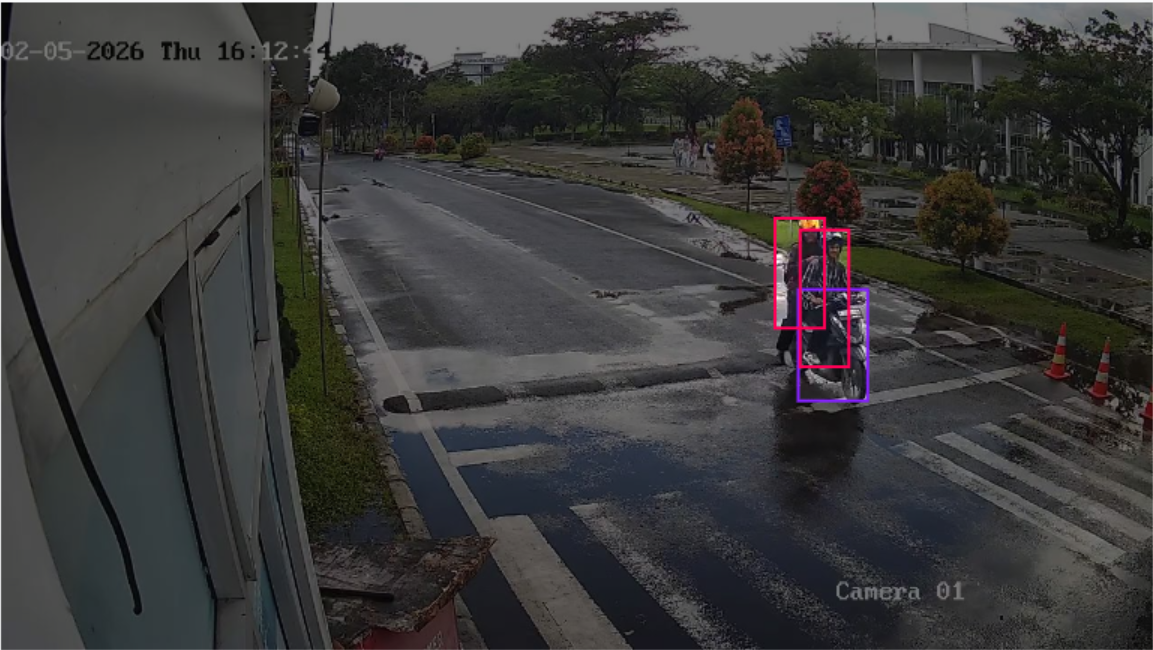
\includegraphics[width=0.8\textwidth]{gambar/data_anotation.png}
  \caption{Contoh anotasi \textit{bounding box} pada pengendara dan sepeda motor dari tangkapan layar CCTV.}
  \label{fig:contoh_anotasi}
\end{figure}

\subsection{Augmentasi Data}
Augmentasi diterapkan hanya pada data latih untuk mengurangi \textit{overfitting} dan meningkatkan generalisasi model. Transformasi meliputi rotasi, \textit{shear}, perubahan eksposur, \textit{blur}, \textit{noise}, dan \textit{motion blur}. Rentang parameter dipilih secara moderat agar variasi visual meningkat tanpa mengubah makna objek. Data validasi dan data uji tidak diaugmentasi untuk menjaga objektivitas evaluasi. Rincian parameter disajikan pada Tabel~\ref{tab:augmentasi}.

\begin{table}[htpb]
  \centering
  \caption{Parameter Augmentasi Data}
  \label{tab:augmentasi}
  \begin{tabular}{ll}
    \toprule
    \textbf{Teknik Augmentasi} & \textbf{Parameter} \\
    \midrule
    Rotation & Antara $-8^\circ$ dan $+8^\circ$ \\
    Shear & $\pm 10^\circ$ horizontal, $\pm 10^\circ$ vertikal \\
    Exposure & Antara $-10\%$ dan $+10\%$ \\
    Blur & Hingga 1,4 piksel \\
    Noise & Hingga 1,09\% dari total piksel \\
    Motion Blur & \textit{Length} 10 px, \textit{Angle} $0^\circ$, \textit{Frames} 1 \\
  \bottomrule
  \end{tabular}
\end{table}

\section{Arsitektur Sistem}
Sistem dibangun dengan \textit{Kappa Architecture} \cite{kreps2014questioning}, yang menempatkan pemrosesan aliran data sebagai jalur utama. Arsitektur ini terdiri atas enam lapisan utama dan ditunjukkan pada Gambar~\ref{fig:architecture}. Secara ringkas, aliran data dimulai dari lapisan \textit{Data Source} sebagai sumber video CCTV yang telah disertai identitas kamera, resolusi, dan posisi geospasial, lalu diteruskan ke lapisan \textit{Ingestion \& Edge Intelligence} untuk akuisisi, pra-pemrosesan \textit{frame}, serta penambahan stempel waktu dan metadata teknis. Data berikutnya dikirim ke lapisan \textit{Buffering} menggunakan Apache Kafka sebagai \textit{message broker} agar aliran data tetap andal, skalabel, dan berurutan per kamera. Setelah itu, lapisan \textit{Stream Processing} memproses \textit{event} secara \textit{real-time} dengan Apache Spark Structured Streaming melalui validasi skema, deduplikasi, dan agregasi singkat sebelum hasilnya disimpan pada lapisan \textit{Persistence} ke dalam \textit{data mart} berdesain skema bintang dengan mekanisme \textit{upsert}. Pada tahap akhir, lapisan \textit{Presentation} memanfaatkan Grafana Dashboard untuk menyajikan hasil analitik secara \textit{real-time} melalui visualisasi yang mendukung pemantauan dan pengambilan keputusan operasional secara cepat dan terarah.

\begin{figure}[H]
  \centering
  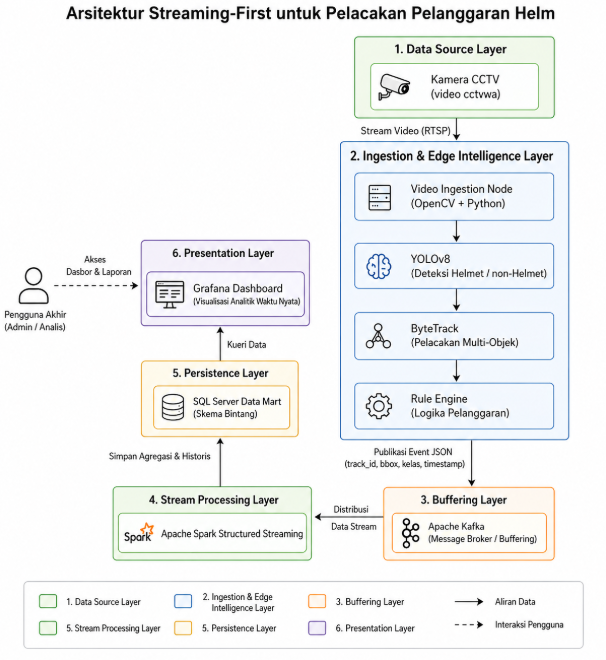
\includegraphics[width=1\textwidth]{gambar/kappa_arsitektur_helm.png}
  \caption{Arsitektur Sistem Streaming-First Pelacakan Pelanggaran Helm}
  \label{fig:architecture}
\end{figure}
\section{Perancangan Model YOLOv8 dan ByteTrack}
Bagian ini menjelaskan perancangan model deteksi dan pelacakan, mulai dari proses pelatihan YOLOv8 hingga integrasi ByteTrack pada tahap inferensi.

\subsection{Pelatihan Model YOLOv8}
Model YOLOv8s yang telah dilatih pada dataset COCO disesuaikan ulang melalui proses \textit{fine-tuning} menggunakan dataset kustom Itera pada \textit{framework} Ultralytics. Proses ini menghasilkan berkas model \textit{best.pt} dengan bobot optimal untuk inferensi pada lapisan \textit{Ingestion \& Edge Intelligence}.

\section{Logika Deteksi Pelanggaran Helm}

Sistem mengintegrasikan model deteksi objek YOLOv8 dan algoritma pelacakan multiobjek ByteTrack untuk mengidentifikasi pengendara yang menggunakan dan tidak menggunakan helm.

Rangkaian proses integrasi sistem adalah sebagai berikut:
\begin{enumerate}[a.]
  \item {Inferensi Deteksi Objek (YOLOv8)}: setiap \textit{frame} video diproses menggunakan model YOLOv8 untuk menghasilkan \textit{bounding box}, label kelas (\texttt{DRIVER\_HELMET}, \texttt{DRIVER\_NO\_HELMET}, dan \texttt{MOTORCYCLE}), serta skor kepercayaan. Deteksi dikonfigurasi dengan parameter \textit{confidence threshold} 0{,}25 dan \textit{NMS IoU threshold} 0{,}7.

  \item {Pelacakan Multi-Objek (ByteTrack)}: hasil deteksi dikirim ke algoritma ByteTrack yang memberikan \texttt{track\_id} persisten pada setiap objek lintas frame. ByteTrack dikonfigurasi dengan \textit{track activation threshold} 0{,}4 (membagi deteksi ke tier tinggi dan rendah), \textit{lost track buffer} 60 \textit{frame} (setara $\approx$2{,}4 detik pada FPS sumber 25 FPS atau $\approx$3{,}17 detik pada FPS efektif \textit{pipeline} 18{,}9 FPS), dan \textit{matching threshold} 0{,}85.

  \item {Asosiasi Spasial Rider--Motorcycle (IoA Filter)}: setelah pelacakan, dilakukan validasi spasial antara deteksi \texttt{DRIVER\_NO\_HELMET} dengan objek \texttt{MOTORCYCLE} menggunakan metrik \textit{Intersection over Area} (IoA). IoA mengukur proporsi area \textit{bounding box} pengendara yang beririsan dengan area motor:
    \begin{equation}
      \text{IoA}(\text{rider}, \text{motor}) = \frac{|\text{bbox}_{\text{rider}} \cap \text{bbox}_{\text{motor}}|}{|\text{bbox}_{\text{rider}}|}
    \end{equation}
    Metrik IoA dipilih ketimbang IoU karena \textit{bounding box} pengendara umumnya jauh lebih kecil daripada motor — IoU akan menghasilkan skor rendah meskipun pengendara jelas berada di atas motor. Pengendara dianggap mengendarai motor jika IoA $\geq$ 0{,}3. Deteksi tanpa asosiasi motor (misalnya pejalan kaki) terfilter pada tahap ini.

  \item {Logika Evaluasi Pelanggaran Helm}: berdasarkan hasil pelacakan dan asosiasi spasial, sistem menerapkan konfirmasi temporal \textit{N-frame} dengan kriteria sebagai berikut:
  \begin{enumerate}[1).]
    \item Label deteksi adalah \texttt{DRIVER\_NO\_HELMET}.
    \item Objek berhasil diasosiasikan secara spasial dengan \texttt{MOTORCYCLE} (IoA $\geq$ 0{,}3).
    \item Status \texttt{DRIVER\_NO\_HELMET} terdeteksi secara berurutan selama setidaknya $N$ frame ($N=3$) untuk menghindari \textit{false positive} akibat \textit{flicker} deteksi.
    \item Mekanisme \textit{patience-based decay}: jika deteksi sesaat hilang (misalnya akibat oklusi parsial), \textit{streak} tidak langsung diatur ulang, melainkan diberi masa tenggang selama \texttt{patience\_frames} (5 frame) sebelum penghapusan.
    \item Skor kepercayaan pelanggaran dihitung sebagai rata-rata \textit{confidence} dari $N$ frame yang terakumulasi, bukan hanya nilai \textit{confidence} pada frame terakhir.
    \item Deduplikasi per-track: setiap \texttt{track\_id} hanya menghasilkan paling banyak satu \textit{event} pelanggaran per sesi untuk menghindari duplikasi.
  \end{enumerate}
\end{enumerate}

\section{Rancangan Basis Data dan Skema Data Mart}
Bagian ini menjelaskan rancangan \textit{data mart} desain skema bintang sebagai dasar analisis pelanggaran.


\subsection{Desain Skema Bintang (Star Schema)}
Pendekatan skema bintang pada Gambar~\ref{fig:stardesign} menempatkan \texttt{fact\_violations} sebagai tabel fakta pusat dan tabel dimensi sebagai pengaya konteks waktu, lokasi, dan jenis pelanggaran. Rancangan ini dipilih karena membuat proses agregasi lebih efisien serta mendukung kebutuhan analisis operasional dan pengembangan dashboard tanpa mengubah struktur data inti.

\begin{figure}[H]
\centering
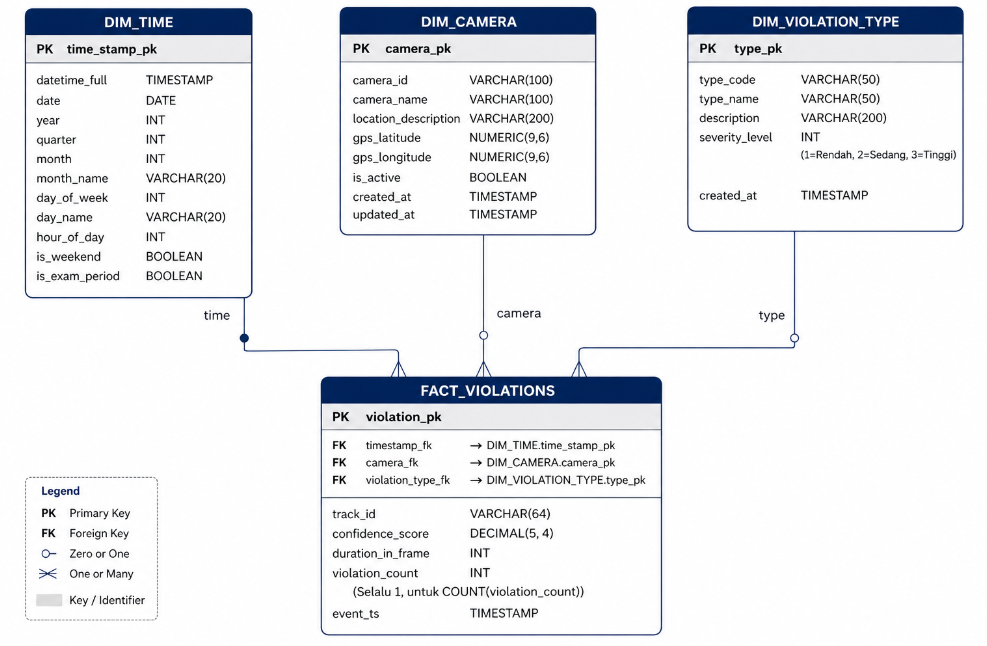
\includegraphics[width=1\textwidth]{gambar/star_schema_helm.png}
\caption{Desain Skema Bintang Data Mart Pelanggaran Helm}
\label{fig:stardesign}
\end{figure}

\section{Rancangan Dashboard Analitik}
Visualisasi hasil deteksi dan pelacakan dirancang dengan \textit{Grafana} yang terhubung ke \textit{data mart} untuk menyajikan ringkasan operasional dan historis secara cepat. Dashboard memuat indikator utama seperti total pelanggaran, jam tersibuk, dan rata-rata jeda antar-pelanggaran, serta analisis tren melalui grafik deret waktu 15 menit, akumulasi harian, dan komposisi periode pagi, siang, dan sore. Selain itu, dashboard juga menampilkan performa sistem dan model melalui distribusi tingkat keyakinan deteksi dan latensi pemrosesan, serta analisis strategis berupa peta panas temporal dan tabel agregat seperti \textit{Top 5 Jam Tersibuk} untuk mendukung pemantauan dan pengambilan keputusan secara lebih efisien.

\section{Alur Penelitian}
\label{sec:alur_penelitian}
Alur penelitian terdiri atas empat tahap utama, mulai dari persiapan data hingga evaluasi sistem (Gambar~\ref{fig:flow-research-systematic}).

\subsection{Tahap 1: Persiapan dan Pra-pemrosesan Data}
Tahap ini menyiapkan dataset dan lingkungan eksperimen untuk pelatihan model visi komputer.
\begin{enumerate}[a.]
\item {Pengumpulan rekaman dan ekstraksi frame selektif}: data primer diperoleh dari rekaman video luring CCTV di gerbang utama Itera. \textit{Frame} diekstraksi secara selektif berdasarkan kualitas visual untuk membentuk \textit{ITERA Helmet Dataset}.
\item {Anotasi objek dan analisis distribusi kelas}: anotasi manual \textit{bounding box} dilakukan pada tiga kelas, yaitu \texttt{DRIVER\_HELMET}, \texttt{DRIVER\_NO\_HELMET}, dan \texttt{MOTORCYCLE}. Distribusi kelas dianalisis untuk mengurangi potensi bias pelatihan.
\item {Pra-pemrosesan dan augmentasi data}: citra distandarkan ke resolusi $640 \times 640$ piksel. Augmentasi geometris dan fotometrik (rotasi, \textit{shear}, eksposur, \textit{noise}, dan \textit{motion blur}) diterapkan untuk meningkatkan generalisasi model.
\end{enumerate}

\subsection{Tahap 2: Pengembangan Model Visi Komputer}
Tahap ini berfokus pada pelatihan dan evaluasi model deteksi objek untuk mengenali atribut keselamatan berkendara.
\begin{enumerate}[a.]
\item {Pelatihan model YOLOv8}: model dilatih selama 300 \textit{epoch} dengan penalaan hiperparameter. Proses pelatihan dipantau melalui \textit{box loss}, \textit{class loss}, dan \textit{distribution focal loss} untuk memastikan konvergensi yang stabil.
\item {Evaluasi kinerja model}: performa model dievaluasi menggunakan mAP@50, \textit{precision}, dan \textit{recall}, baik secara agregat maupun per kelas.
\end{enumerate}

\subsection{Tahap 3: Konstruksi Pipeline Streaming Real-Time}
Tahap ini membangun pipeline streaming terdistribusi untuk mengubah deteksi mentah menjadi \textit{event} terverifikasi.
\begin{enumerate}[a.]
\item {Integrasi inferensi dan pelacakan}: inferensi YOLOv8 diintegrasikan dengan pelacakan multiobjek ByteTrack pada sisi \textit{edge} untuk menjaga identitas kendaraan (\textit{Track ID}) secara persisten.
\item {Penerapan filter logika bertingkat}: metrik IoA digunakan untuk memvalidasi asosiasi antara pengendara dan sepeda motor, lalu konfirmasi temporal \textit{N-frame} diterapkan untuk menekan \textit{false positive} akibat oklusi sesaat.
\item {Serialisasi dan transmisi pesan}: data anomali yang lolos validasi dikemas dalam \textit{payload} JSON dan dikirim melalui Apache Kafka dengan kunci partisi \texttt{camera\_id:track\_id} agar domain urutan kejadian tetap konsisten per kamera.
\item {Pemrosesan ETL streaming}: Apache Spark Structured Streaming mengonsumsi \textit{event} dari Kafka, melakukan \textit{micro-batching}, deduplikasi berbasis \texttt{event\_id} dengan watermark 30 detik, serta ekstraksi dimensi waktu sebelum pemuatan idempotent ke PostgreSQL melalui mekanisme \textit{upsert}.
\item {Evaluasi kinerja pipeline}: efisiensi sistem diukur melalui \textit{throughput} (\textit{frame} per detik) dan latensi pemrosesan pada setiap subsistem.
\end{enumerate}

\subsection{Tahap 4: Implementasi Data Mart dan Visualisasi}
Tahap terakhir mengonsolidasikan data operasional ke \textit{data mart} analitik dan mengevaluasi fungsionalitas akhir sistem.
\begin{enumerate}[a.]
\item {Pemuatan data ke skema bintang}: data dimuat ke PostgreSQL dengan desain \textit{star schema}. Skema ini memisahkan tabel fakta (\texttt{fact\_violations}) dan tabel dimensi (\texttt{dim\_camera}, \texttt{dim\_time}, \texttt{dim\_violation\_type}) untuk mempercepat kueri agregasi.
\item {Visualisasi dasbor analitik}: antarmuka pemantauan dibangun di Grafana yang terhubung langsung ke \textit{data mart} untuk menyajikan metrik operasional secara interaktif.
\end{enumerate}

\begin{figure}[p]
\centering
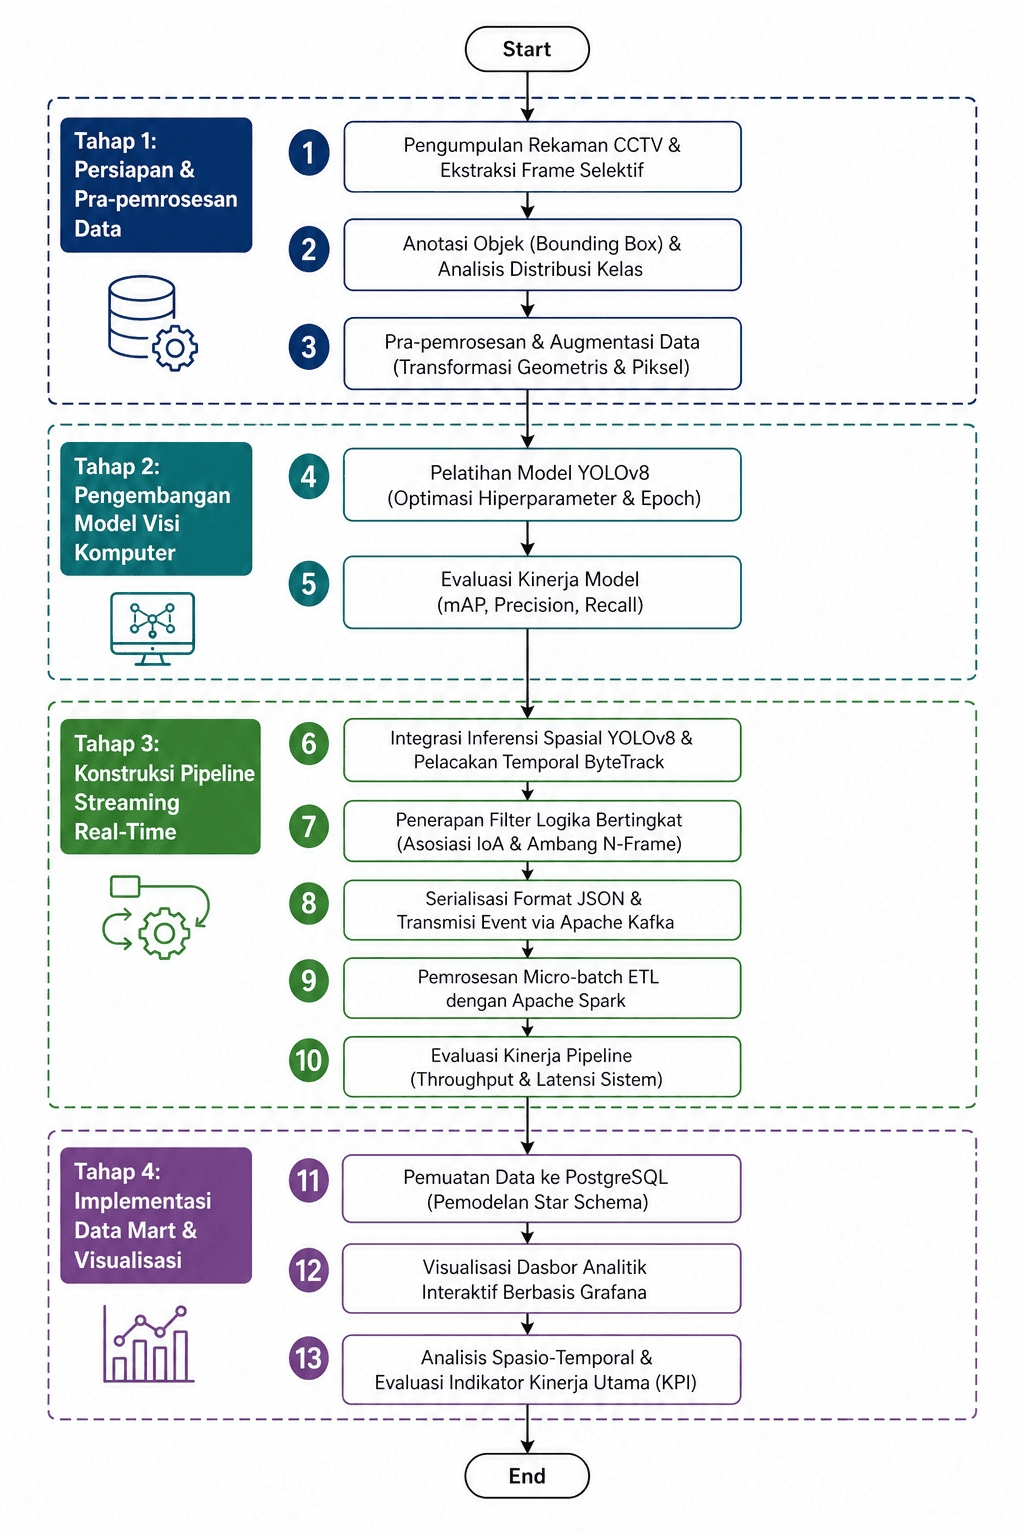
\includegraphics[width=0.8\textwidth,height=0.78\textheight,keepaspectratio]{gambar/alur penelitian.png}
\caption{Diagram Alur Penelitian Sistem Pelacakan Pelanggaran Helm}
\label{fig:flow-research-systematic}
\end{figure}
